\documentclass[compress]{beamer}

\usepackage[T1,T2A]{fontenc}
\usepackage[utf8]{inputenc}
\usepackage[english,russian]{babel}
\usepackage{hyperref}
\usepackage{microtype}
\usepackage{csquotes}
\usepackage{amsmath}
\usepackage{amsthm}
\usepackage{amssymb}
\usepackage{mathtext}
\usepackage{physics}
\usepackage{newfloat}
\usepackage{caption}
\usepackage{indentfirst}
\usepackage{hyperref}
\usepackage{mdframed}
\usepackage{graphicx}
\usepackage{subfig}
\usepackage{appendix}

%% workaround for the \@ifundefined macro update in the 2018 LaTeX release
%% should be fixed in one of the next releases of caption.sty
\makeatletter
\let\@@magyar@captionfix\relax
\makeatother

\DeclareGraphicsExtensions{.pdf,.png,.jpg,.PNG}
\graphicspath{{./img/}}
\captionsetup[figure]{justification=centering}
\renewcommand{\thesubfigure}{\asbuk{subfigure}}
\DeclareCaptionLabelSeparator{dotseparator}{. }
\captionsetup{labelsep=dotseparator}
\makeatletter\appto{\appendices}{\def\Hy@chapapp{Appendix}}\makeatother
\renewcommand{\appendixtocname}{Приложения}
\renewcommand{\appendixpagename}{Приложения}
\setbeamertemplate{background canvas}[vertical shading][bottom=red!2,top=green!2]

\usetheme{Ilmenau}
\usecolortheme{spruce}
\usefonttheme[onlysmall]{serif}

\setbeamercolor{title in head/foot}{parent=palette primary}
\setbeamercolor{author in head/foot}{parent=palette primary}
\setbeamercolor{institute in head/foot}{parent=palette primary}

\setbeamercolor{title}{fg=black}
\setbeamercolor{frametitle}{fg=black}
\setbeamercolor*{enumerate item}{fg=black}

\setbeamercolor*{bibliography item}{fg=black}
\setbeamercolor*{bibliography entry title}{fg=black}
\setbeamercolor*{bibliography entry author}{fg=black}
\setbeamercolor*{bibliography entry location}{fg=black}
\setbeamercolor*{bibliography entry note}{fg=black}

\setbeamertemplate{enumerate item}[default]
\setbeamertemplate{bibliography entry title}{}
\setbeamertemplate{bibliography entry location}{}
\setbeamertemplate{bibliography entry note}{}
\setbeamertemplate{bibliography item}{\insertbiblabel}

\addtobeamertemplate{navigation symbols}{}{%
    \usebeamerfont{footline}%
    \usebeamercolor[fg]{title}%
    \hspace{1em}%
    \insertframenumber/\inserttotalframenumber
}

\hypersetup{
    colorlinks,
    citecolor=black,
    filecolor=black,
    linkcolor=black,
    urlcolor=black
}

\AtBeginSection[]{
  \begin{frame}
  \vfill
  \centering
  \begin{beamercolorbox}[sep=8pt,center,shadow=true,rounded=true]{title}
    \usebeamerfont{title}\insertsection\par%
  \end{beamercolorbox}
  \vfill
  \end{frame}
}

\DeclareMathOperator{\Rot}{\mathbf{rot}}
\DeclareMathOperator{\Grad}{\mathbf{grad}}
\DeclareMathOperator{\Div}{\mathbf{div}}
\DeclareMathOperator{\D}{D}
\newcommand{\V}[1]{\mathbf{#1}}
\newcommand{\Op}[1]{\hat{\V{#1}}}


\graphicspath{{./img/}{../../fragments/math/img/}{../../fragments/spherical_modes/img/}{../../fragments/spherical_resonators/img/}{../../fragments/thermodynamics/img/}}

\deftranslation[to=russian]{Theorem}{Теорема}
\deftranslation[to=russian]{theorem}{Теорема}

\title{Тепловое излучение\\ в сферическом резонаторе}
\author[Василевский~А.В.]{
    Василевский~А.В. \\[\baselineskip]
    {\footnotesize Научный руководитель: Бурланков~Д.Е.}
}
\institute[ННГУ]{Нижегородский университет им. Н.И.~Лобачевского}
\date{2018}

\begin{document}

    %
    %
    %
    %%%%%%%%%%%%%%%%%%%%%%%%%%%%%%%%%%%%%%%%%%%%%%%%%%%%%%%%%%%%%%%%%%%%%%%
    %                            FRAME                                    %
    %%%%%%%%%%%%%%%%%%%%%%%%%%%%%%%%%%%%%%%%%%%%%%%%%%%%%%%%%%%%%%%%%%%%%%%
    %
    %
    %

    \frame[plain]{\titlepage}

    %
    %
    %
    %%%%%%%%%%%%%%%%%%%%%%%%%%%%%%%%%%%%%%%%%%%%%%%%%%%%%%%%%%%%%%%%%%%%%%%
    %                            FRAME                                    %
    %%%%%%%%%%%%%%%%%%%%%%%%%%%%%%%%%%%%%%%%%%%%%%%%%%%%%%%%%%%%%%%%%%%%%%%
    %
    %
    %

    \begin{frame}\frametitle{Постановка задачи}

        \textbf{Цели работы}:
        %
        \begin{itemize}\justifying
            \item \textbf{Описание теплового излучения внутри сферического резонатора}.
                Применен подход, в основе которого лежат векторы Киллинга объемлющего пространства.
            \item \textbf{Описание энергии теплового излучения в сферическом резонаторе}.
                Энергетический спектр дискретен. Важен вклад конкретных мод. Переход к планковскому спектру возможен лишь при больших частотах.
        \end{itemize}

        \textbf{Физическая модель резонатора}:
        %
        \begin{itemize}\justifying
            \item Идеально сферический радиуса $R$.
            \item Заполнен изотропным однородным диэлектриком.
            \item Стенки идеально проводящие.
        \end{itemize}

    \end{frame}

    %
    %
    %
    %%%%%%%%%%%%%%%%%%%%%%%%%%%%%%%%%%%%%%%%%%%%%%%%%%%%%%%%%%%%%%%%%%%%%%%
    %                            FRAME                                    %
    %%%%%%%%%%%%%%%%%%%%%%%%%%%%%%%%%%%%%%%%%%%%%%%%%%%%%%%%%%%%%%%%%%%%%%%
    %
    %
    %

    \begin{frame}\frametitle{Волновое уравнение}

        \begin{itemize}\justifying

            \item Основное уравнение задачи~--- волновое уравнение для комплексной амплитуды вектора напряженности $\V{E}$:
            %
            \begin{gather}
                \vb{E}_{osc} = \Re{\vb{E} \exp(-i \omega t)} \nonumber \\
                \Delta \V{E} = - \lambda \V{E} ; \quad
                    \lambda = \frac{\omega^2}{v^2} ; \quad
                    v = \frac{c}{\sqrt{\varepsilon\mu}} = \frac{c}{n} \label{eq:wave_equation}.
            \end{gather}

            \item Уравнение \autoref{eq:wave_equation}~--- уравнение на собственные функции и собственные значения (моды) оператора Лапласа $\Delta$.

            \item Поскольку стенки резонатора~--- идеальные проводники, то граничные условия: $\vb{E}^\theta = \vb{E}^\varphi = 0$ при $r = R$.

        \end{itemize}

    \end{frame}

    %
    %
    %
    %%%%%%%%%%%%%%%%%%%%%%%%%%%%%%%%%%%%%%%%%%%%%%%%%%%%%%%%%%%%%%%%%%%%%%%
    %                            FRAME                                    %
    %%%%%%%%%%%%%%%%%%%%%%%%%%%%%%%%%%%%%%%%%%%%%%%%%%%%%%%%%%%%%%%%%%%%%%%
    %
    %
    %

    \begin{frame}\frametitle{Операторы вращений}

        \begin{itemize}\justifying

            \item Поле Киллинга~--- векторное поле, сдвиг по которому (Ли-вариация, оператор Киллинга) не изменяет метрический тензор.

            \item Операторы Киллинга коммутируют с оператором Лапласа.

            \item $\qty{ \V{l}_x, \V{l}_y, \V{l}_z }$~--- поля Киллинга вращений трехмерного евклидова пространства.

            \item Оператор $\Op{l}^2 = \Op{l}_x \Op{l}_x + \Op{l}_y \Op{l}_y + \Op{l}_z \Op{l}_z$ коммутирует со всеми операторами вращений.

            \item Операторы повышения и понижения, $\Op{l}_{+} = \Op{l}_x - i\Op{l}_y$ и $\Op{l}_{-} = \Op{l}_x + i\Op{l}_y$, также коммутируют с $\Op{l}^2$.

        \end{itemize}

    \end{frame}

    %
    %
    %
    %%%%%%%%%%%%%%%%%%%%%%%%%%%%%%%%%%%%%%%%%%%%%%%%%%%%%%%%%%%%%%%%%%%%%%%
    %                            FRAME                                    %
    %%%%%%%%%%%%%%%%%%%%%%%%%%%%%%%%%%%%%%%%%%%%%%%%%%%%%%%%%%%%%%%%%%%%%%%
    %
    %
    %

    \begin{frame}\frametitle{Собственные моды операторов вращений}

        Рассмотрим некоторую собственную для $\Op{l}^2$ и $\Op{l}_z$ моду $h_{l,m}$:
        %
        \begin{alignat*}{3}
            \Op{l}^2 h_{l,m} &= &{}- l (l + 1) &\ h_{l,m} , \\
            \Op{l}_z h_{l,m} &= &{}i m         &\ h_{l,m} .
        \end{alignat*}

        Можно показать, что
        %
        \begin{equation*}\begin{aligned}
            \Op{l}_{+} h_{l,m} &= h_{l,m+1} , \\
            \Op{l}_{-} h_{l,m} &= h_{l,m-1}
        \end{aligned}\end{equation*}
        %
        и что $- l \le m \le l$.

    \end{frame}

    %
    %
    %
    %%%%%%%%%%%%%%%%%%%%%%%%%%%%%%%%%%%%%%%%%%%%%%%%%%%%%%%%%%%%%%%%%%%%%%%
    %                            FRAME                                    %
    %%%%%%%%%%%%%%%%%%%%%%%%%%%%%%%%%%%%%%%%%%%%%%%%%%%%%%%%%%%%%%%%%%%%%%%
    %
    %
    %

    \begin{frame}\frametitle{Базовые моды}

        Легко убедиться, что базовая мода,  т.е. мода с $m = 0$, не зависит от $\varphi$:
        %
        \begin{equation*}
            \Op{l}_z h_{l, 0} = \pdv{\varphi} h_{l, 0} \overset{\left\{\text{по смыслу $m$}\right\}}{=} 0 .
        \end{equation*}
        %
        Кроме того, базовая мода удовлетворяет соотношению:
        %
        \begin{equation}\begin{aligned}\label{eq:basemode_eq}
            \Op{l}^2 h_{l, 0}
                &= \qty( \Op{l}_{+} \Op{l}_{-} + \Op{l}_z^2 - i \Op{l}_z ) h_{l, 0} \\
                &= \Op{l}_{+} \Op{l}_{-} h_{l, 0}
                 = - l (l + 1) h_{l, 0} .
        \end{aligned}\end{equation}
        %
        Но поскольку $\Op{l}_i$ не содержит $r$, уравнение \autoref{eq:basemode_eq} является уравнением только на $h_{l, 0}$ как функцию $\theta$.

    \end{frame}

    %
    %
    %
    %%%%%%%%%%%%%%%%%%%%%%%%%%%%%%%%%%%%%%%%%%%%%%%%%%%%%%%%%%%%%%%%%%%%%%%
    %                            FRAME                                    %
    %%%%%%%%%%%%%%%%%%%%%%%%%%%%%%%%%%%%%%%%%%%%%%%%%%%%%%%%%%%%%%%%%%%%%%%
    %
    %
    %

    \begin{frame}\frametitle{Методика нахождения сферических мод}

        \begin{enumerate}\justifying
            \item Нахождение угловых частей базовых мод с $m = 0$ и определенным $l$ из \autoref{eq:basemode_eq}:
            %
            \begin{equation*}
                \Op{l}_{+} \Op{l}_{-} h_{l, 0} = - l (l + 1) h_{l, 0} .
            \end{equation*}

            \item Нахождение радиальных функций для базовых мод из \autoref{eq:wave_equation}:
            %
            \begin{equation*}
                \Delta h_{l, 0} = - \lambda h_{l, 0} .
            \end{equation*}

            \item Получение остальных $2l$ производных мод с $m = \pm 1, \pm 2, \dots$ путем применения операторов повышения и понижения.

        \end{enumerate}

    \end{frame}

    %
    %
    %
    %%%%%%%%%%%%%%%%%%%%%%%%%%%%%%%%%%%%%%%%%%%%%%%%%%%%%%%%%%%%%%%%%%%%%%%
    %                            FRAME                                    %
    %%%%%%%%%%%%%%%%%%%%%%%%%%%%%%%%%%%%%%%%%%%%%%%%%%%%%%%%%%%%%%%%%%%%%%%
    %
    %
    %

    \begin{frame}\frametitle{Поляризации векторных мод}

        Можно показать, что возможны две поляризации векторного поля $\vb{a}$, удовлетворяющие волновому уравнению:
        %
        \begin{equation*}\begin{gathered}
            \vb{a}_{\mathrm{I}} = \qty{ a^r, a^\theta, 0 } , \quad
            \vb{a}_{\mathrm{II}} = \qty{ 0, 0, a^\varphi } , \quad \text{причем} \\
            \Rot\vb{a}_{\mathrm{I}} = \vb{a}_{\mathrm{II}}
        \end{gathered}\end{equation*}

        Применительно к электромагнитному полю конфигурации $\vb{E} = \qty{ E^r, E^\theta, 0 }$ и $\vb{E} = \qty{ 0, 0, E^\varphi }$ называются соответственно $TH$ и $TE$.

    \end{frame}

    %
    %
    %
    %%%%%%%%%%%%%%%%%%%%%%%%%%%%%%%%%%%%%%%%%%%%%%%%%%%%%%%%%%%%%%%%%%%%%%%
    %                            FRAME                                    %
    %%%%%%%%%%%%%%%%%%%%%%%%%%%%%%%%%%%%%%%%%%%%%%%%%%%%%%%%%%%%%%%%%%%%%%%
    %
    %
    %

    \begin{frame}\frametitle{Векторные моды}

        Опуская математические выкладки, запишем вид $\vb{E}_{TE}$:
        %
        \begin{equation}\label{eq:ete}
            \vb{E}_{TE} = \begin{pmatrix}
                0 \\ 0 \\ \flatfrac{S_l(\sqrt\lambda r)}{r^2} \csc(\theta) P^1_l(\cos\theta)
            \end{pmatrix} .
        \end{equation}
        %
        Применением ротора к \autoref{eq:ete} получим $\vb{E}_{TH}$:
        %
        \begin{equation}\label{eq:eth}
            \vb{E}_{TH} = \begin{pmatrix}
                \flatfrac{l(l+1) S_l(\sqrt\lambda r)}{r^2} P_l(\cos\theta) \\
                \flatfrac{S_l'(\sqrt\lambda r)}{r^2} P_l^1(\cos\theta) \\
                0
            \end{pmatrix} .
        \end{equation}

    \end{frame}

    %
    %
    %
    %%%%%%%%%%%%%%%%%%%%%%%%%%%%%%%%%%%%%%%%%%%%%%%%%%%%%%%%%%%%%%%%%%%%%%%
    %                            FRAME                                    %
    %%%%%%%%%%%%%%%%%%%%%%%%%%%%%%%%%%%%%%%%%%%%%%%%%%%%%%%%%%%%%%%%%%%%%%%
    %
    %
    %

    \begin{frame}

        \begin{figure}[h]
            \centering
            %
            \subfloat[][]{%
                \label{fig:angle_modes_vect_ii}%
                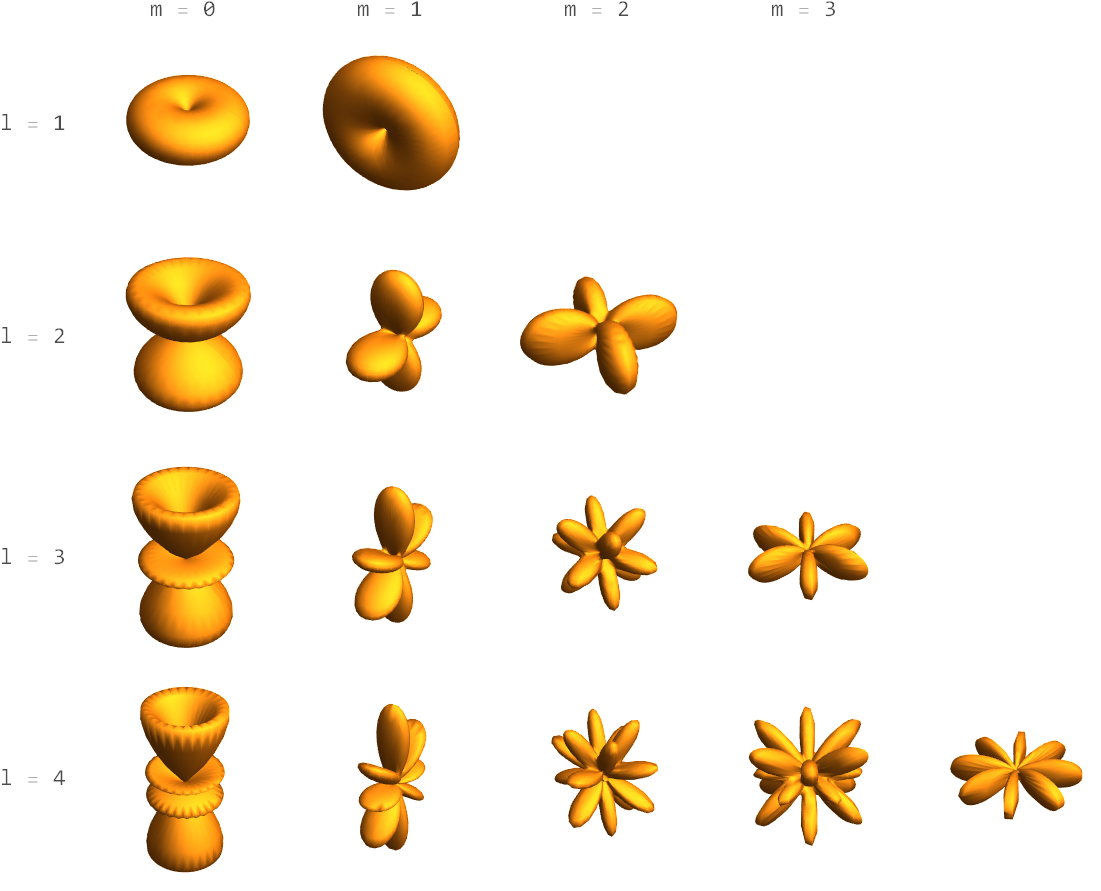
\includegraphics[width=0.5\textwidth]{angle_modes_vect_ii}}%
            %
            \subfloat[][]{%
                \label{fig:radial_modes_vect_ii}%
                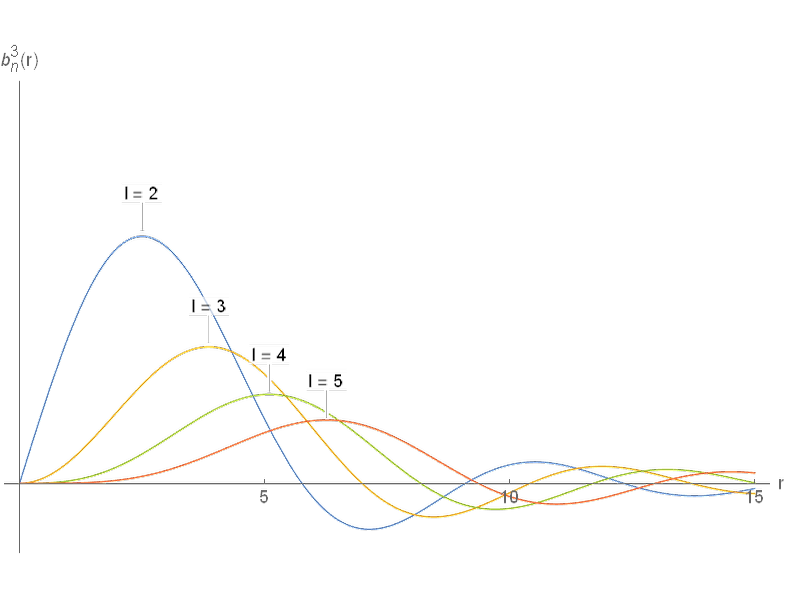
\includegraphics[width=0.5\textwidth]{radial_modes_vect_ii}}%
            %
            \caption[]{Векторные угловые (изображена плотность энергии) и радиальные моды для нескольких $l$}
        \end{figure}

    \end{frame}

    %
    %
    %
    %%%%%%%%%%%%%%%%%%%%%%%%%%%%%%%%%%%%%%%%%%%%%%%%%%%%%%%%%%%%%%%%%%%%%%%
    %                            FRAME                                    %
    %%%%%%%%%%%%%%%%%%%%%%%%%%%%%%%%%%%%%%%%%%%%%%%%%%%%%%%%%%%%%%%%%%%%%%%
    %
    %
    %

    \begin{frame}\frametitle{Учет граничных условий}

        \begin{itemize}\justifying
            \item Поверхность резонатора~--- идеальный проводник.

            \item В силу этого $E^\varphi = E^\theta = 0$ при $r = R$.

            \item Отсюда из \autoref{eq:ete} и \autoref{eq:eth} радиальные функции должны обращаться в нуль при $r = R$.

            \item Таким образом, из граничных условий получим спектр собственных частот резонатора $\omega^{lp}_n$ ($p$~--- тип поляризации, $TH$ или $TE$).

            \item $\omega^{lp}_n$-й собственной частоте соответствует $2l + 1$ мод (одна базовая с $m = 0$ и $2l$ производных с $m = \pm 1, \pm 2, \dots, \pm l$).
        \end{itemize}

    \end{frame}

    %
    %
    %
    %%%%%%%%%%%%%%%%%%%%%%%%%%%%%%%%%%%%%%%%%%%%%%%%%%%%%%%%%%%%%%%%%%%%%%%
    %                            FRAME                                    %
    %%%%%%%%%%%%%%%%%%%%%%%%%%%%%%%%%%%%%%%%%%%%%%%%%%%%%%%%%%%%%%%%%%%%%%%
    %
    %
    %

    \begin{frame}\frametitle{Спектральная плотность энергии}

        \begin{itemize}\justifying

            \item По определению спектральной плотности энергии
            %
            \begin{equation}\label{eq:psd}
                u(\omega) \dd{\omega} = \hbar\omega\ n(\hbar\omega) \dd{N(\omega)} ,
            \end{equation}

            \item Распределение Бозе-Эйнштейна~--- среднее число фотонов с данной энергией $\varepsilon = \hbar\omega$ в каждой моде:
            %
            \begin{equation}\label{eq:n_of_eps}
                n(\varepsilon) = \frac{1}{\exp(\flatfrac{\varepsilon}{kT}) - 1} .
            \end{equation}

        \end{itemize}

    \end{frame}

    %
    %
    %
    %%%%%%%%%%%%%%%%%%%%%%%%%%%%%%%%%%%%%%%%%%%%%%%%%%%%%%%%%%%%%%%%%%%%%%%
    %                            FRAME                                    %
    %%%%%%%%%%%%%%%%%%%%%%%%%%%%%%%%%%%%%%%%%%%%%%%%%%%%%%%%%%%%%%%%%%%%%%%
    %
    %
    %

    \begin{frame}\frametitle{Формула Планка}

        \begin{itemize}\justifying

            \item Можно показать \cite{sivuhin_opt}, что для электромагнитного поля
            %
            \begin{equation}\label{eq:dN_of_eps_cont}
                \dd{N(\omega)} = \frac{\omega^2 \dd{\omega}}{\pi^2 v^3} \quad
                    \text{при больших $\omega$}.
            \end{equation}

            \item Формула Планка:
            %
            \begin{equation}
                u(\omega) = \frac{
                        \flatfrac{\omega^2 \hbar\omega}{\pi^2 v^3}
                }{\exp(\flatfrac{\hbar\omega}{kT}) - 1} .
            \end{equation}

            \item В сферическом резонаторе спектр дискретный,
            %
            \begin{equation*}
                N(\omega^{lp}_n) = V^{-1} (2l + 1) .
            \end{equation*}

        \end{itemize}

    \end{frame}

    %
    %
    %
    %%%%%%%%%%%%%%%%%%%%%%%%%%%%%%%%%%%%%%%%%%%%%%%%%%%%%%%%%%%%%%%%%%%%%%%
    %                            FRAME                                    %
    %%%%%%%%%%%%%%%%%%%%%%%%%%%%%%%%%%%%%%%%%%%%%%%%%%%%%%%%%%%%%%%%%%%%%%%
    %
    %
    %

    \begin{frame}\frametitle{Энергетический спектр}

        \begin{itemize}\justifying
            \item Интегральная энергия складывается из:
            %
            \begin{equation*}
                W = \int u(\omega) \dd{\omega} = \sum \hbar\omega_n\ n(\hbar\omega_n) N(\omega_n) = \sum W_n .
            \end{equation*}

            \item При $T \to \infty$~--- равномерное распределение энергии
            %
            \begin{equation*}
                W^{lp}_n \approx N(\omega^{lp}_n) kT .
            \end{equation*}

            \item При $T \to 0$~--- формула Вина для отдельно взятой моды
            %
            \begin{equation*}
                W^{lp}_n \approx \hbar\omega^{lp}_n \exp(-\flatfrac{\hbar\omega^{lp}_n}{kT}) N(\omega^{lp}_n) .
            \end{equation*}

        \end{itemize}

    \end{frame}

    %
    %
    %
    %%%%%%%%%%%%%%%%%%%%%%%%%%%%%%%%%%%%%%%%%%%%%%%%%%%%%%%%%%%%%%%%%%%%%%%
    %                            FRAME                                    %
    %%%%%%%%%%%%%%%%%%%%%%%%%%%%%%%%%%%%%%%%%%%%%%%%%%%%%%%%%%%%%%%%%%%%%%%
    %
    %
    %

    \begin{frame}

        \begin{figure}[h]
            \centering
            \begin{tabular}{ l c r }
                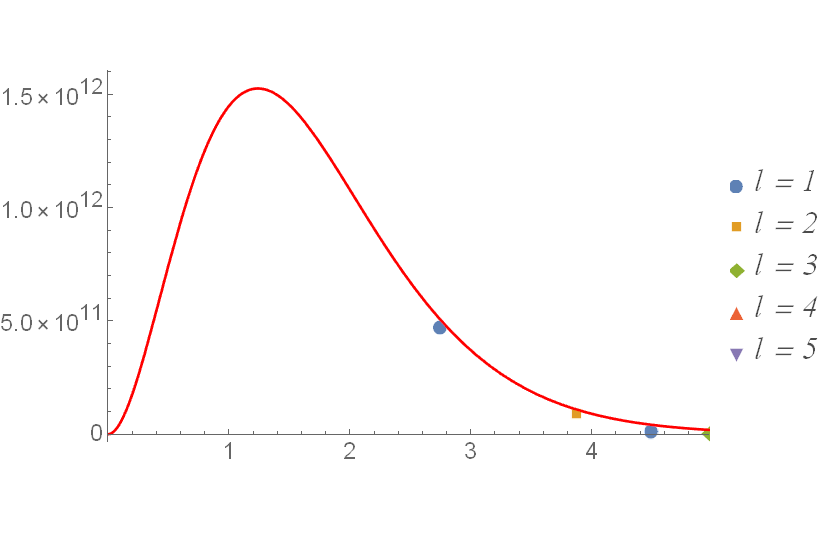
\includegraphics[width=0.5\textwidth]{plank_small_t_1} & 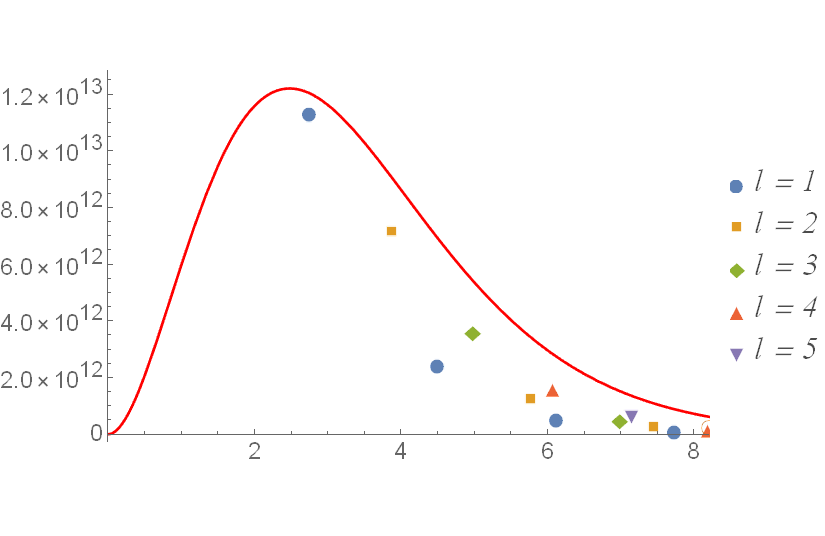
\includegraphics[width=0.5\textwidth]{plank_small_t_2} \\
                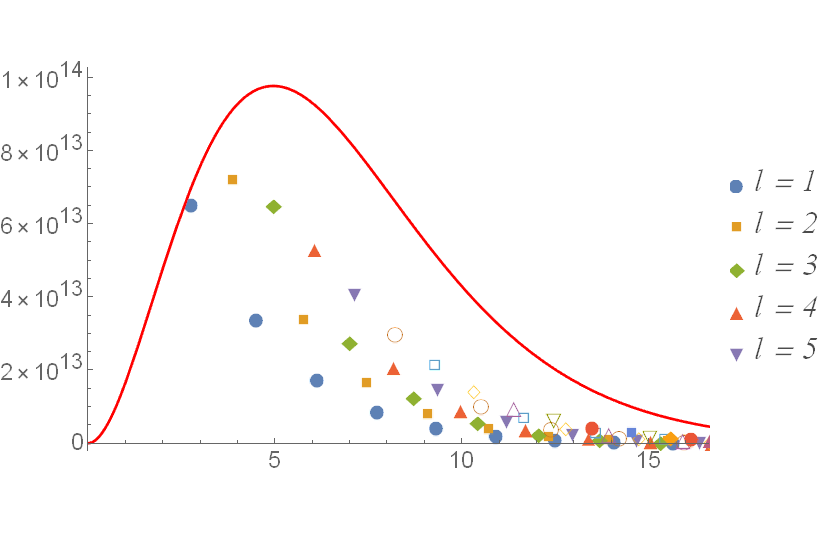
\includegraphics[width=0.5\textwidth]{plank_small_t_3} & 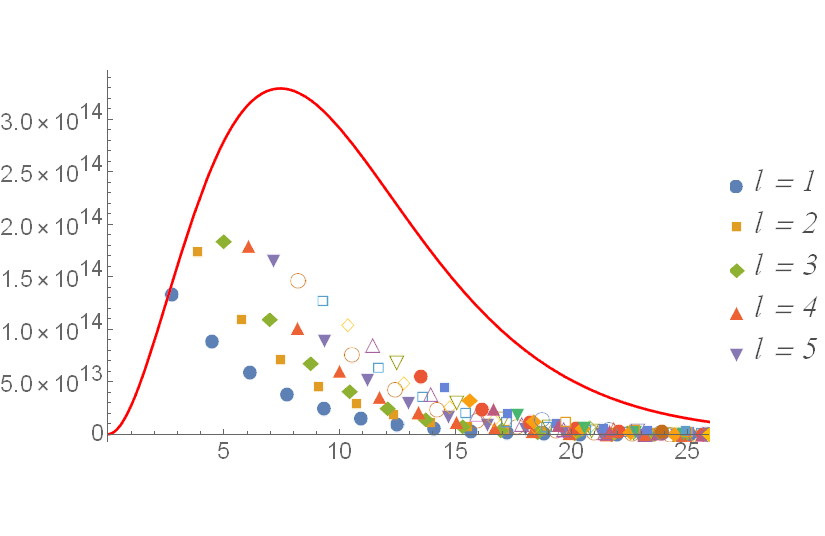
\includegraphics[width=0.5\textwidth]{plank_small_t_4} \\
            \end{tabular}
        \end{figure}

    \end{frame}

    %
    %
    %
    %%%%%%%%%%%%%%%%%%%%%%%%%%%%%%%%%%%%%%%%%%%%%%%%%%%%%%%%%%%%%%%%%%%%%%%
    %                            FRAME                                    %
    %%%%%%%%%%%%%%%%%%%%%%%%%%%%%%%%%%%%%%%%%%%%%%%%%%%%%%%%%%%%%%%%%%%%%%%
    %
    %
    %

    \begin{frame}\frametitle{Область высоких частот}

        Собственные частоты расположены плотно. Можно совершить переход к непрерывным величинам, заменяя $\dd{N(\omega)}$ на $\Delta N(\omega)$.

        \begin{figure}[h]
            \centering
            %
            \subfloat[][]{%
                \label{fig:n_full}%
                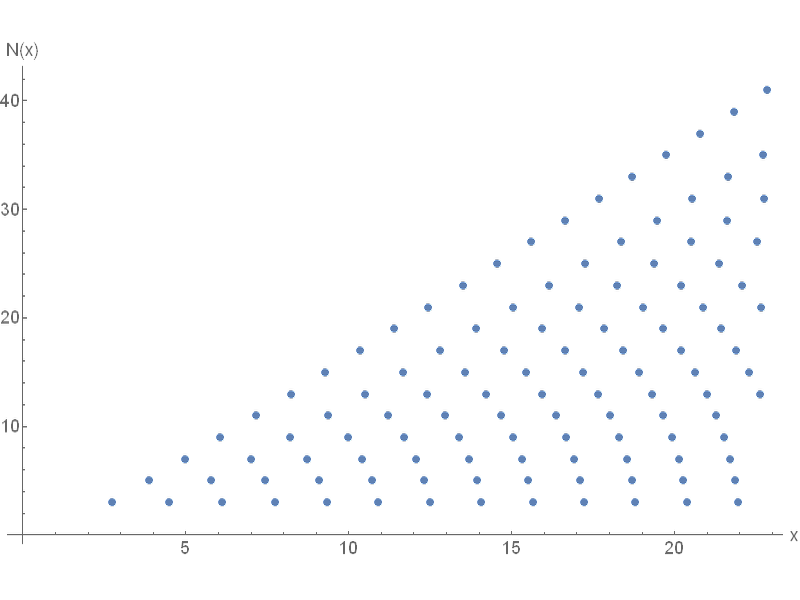
\includegraphics[width=0.33\textwidth]{n_full}}%
            %
            \subfloat[][]{%
                \label{fig:dndx}%
                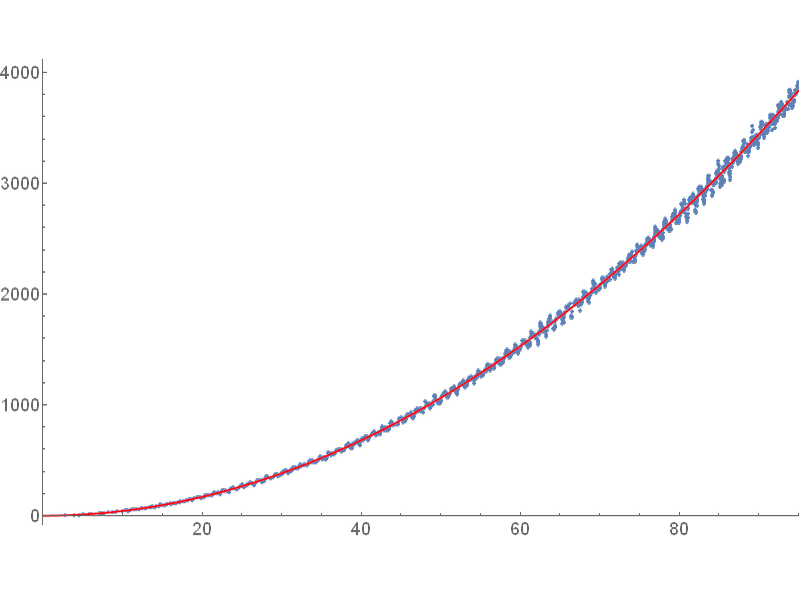
\includegraphics[width=0.33\textwidth]{dndx}}%
            %
            \subfloat[][]{%
                \label{fig:plank}%
                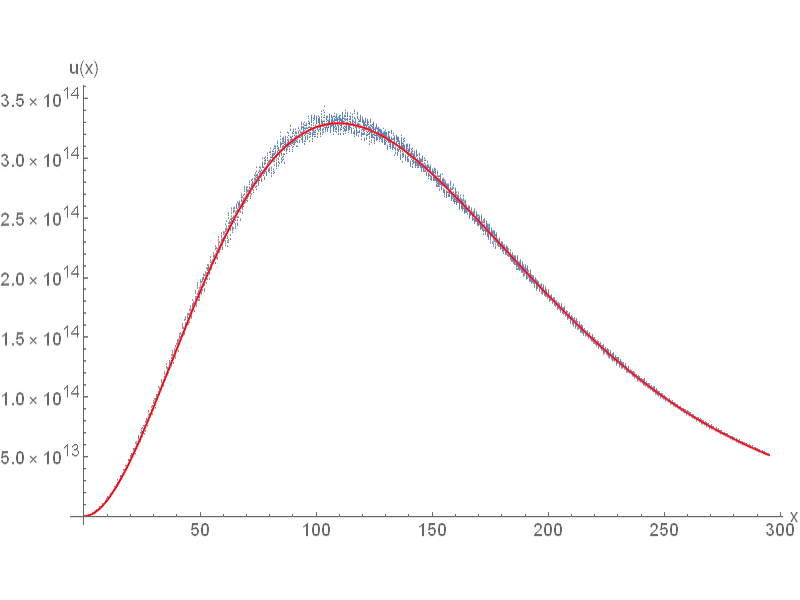
\includegraphics[width=0.33\textwidth]{plank}}%
            %
            \caption[]{\subref{fig:n_full} $N(x_n)$, \subref{fig:dndx} $\flatfrac{\Delta N}{\Delta x}$ (синим, точки) и $\dv*{N}{x}$ (красным), \subref{fig:plank} кривая планка, построенная на $\flatfrac{\Delta N}{\Delta x}$ (синим, точки) и на $\dv*{N}{x}$ (красным). Величина $x = \flatfrac{\omega}{v} R$}
        \end{figure}

    \end{frame}

    %
    %
    %
    %%%%%%%%%%%%%%%%%%%%%%%%%%%%%%%%%%%%%%%%%%%%%%%%%%%%%%%%%%%%%%%%%%%%%%%
    %                            FRAME                                    %
    %%%%%%%%%%%%%%%%%%%%%%%%%%%%%%%%%%%%%%%%%%%%%%%%%%%%%%%%%%%%%%%%%%%%%%%
    %
    %
    %

    \begin{frame}\frametitle{Заключение}

        \begin{itemize}\justifying
            \item В работе продемонстрировано применение методики Ли-генерации мод скалярного и векторного полей в трехмерном евклидовом пространстве.

            \item Математические выкладки проделаны для риманова пространства общего вида.

            \item Получен вид скалярных и векторных сферических мод.

            \item Рассмотрен энергетический спектр электромагнитного поля в резонаторе при различных температурах.

            \item Совершен асимптотический переход к планковскому спектру.
        \end{itemize}

        Все поставленные цели были достигнуты.

    \end{frame}

    %
    %
    %
    %%%%%%%%%%%%%%%%%%%%%%%%%%%%%%%%%%%%%%%%%%%%%%%%%%%%%%%%%%%%%%%%%%%%%%%
    %                        BIBLIOGRAPHY                                 %
    %%%%%%%%%%%%%%%%%%%%%%%%%%%%%%%%%%%%%%%%%%%%%%%%%%%%%%%%%%%%%%%%%%%%%%%
    %
    %
    %

    \begin{frame}\frametitle{Литература}
        \nocite{burlankov_tmf,methods_of_theoretical_physics}
        \bibliographystyle{../../../lib/doc/bib/utf8gost705s}
        \bibliography{%
            ../../../lib/doc/bib/resonators,%
            ../../../lib/doc/bib/physics,%
            ../../../lib/doc/bib/math%
        }
    \end{frame}

\end{document}
